% Options for packages loaded elsewhere
\PassOptionsToPackage{unicode}{hyperref}
\PassOptionsToPackage{hyphens}{url}
\PassOptionsToPackage{dvipsnames,svgnames,x11names}{xcolor}
%
\documentclass[
  a4paper,
  DIV=11,
  numbers=noendperiod]{scrreprt}

\usepackage{amsmath,amssymb}
\usepackage{iftex}
\ifPDFTeX
  \usepackage[T1]{fontenc}
  \usepackage[utf8]{inputenc}
  \usepackage{textcomp} % provide euro and other symbols
\else % if luatex or xetex
  \usepackage{unicode-math}
  \defaultfontfeatures{Scale=MatchLowercase}
  \defaultfontfeatures[\rmfamily]{Ligatures=TeX,Scale=1}
\fi
\usepackage{lmodern}
\ifPDFTeX\else  
    % xetex/luatex font selection
\fi
% Use upquote if available, for straight quotes in verbatim environments
\IfFileExists{upquote.sty}{\usepackage{upquote}}{}
\IfFileExists{microtype.sty}{% use microtype if available
  \usepackage[]{microtype}
  \UseMicrotypeSet[protrusion]{basicmath} % disable protrusion for tt fonts
}{}
\makeatletter
\@ifundefined{KOMAClassName}{% if non-KOMA class
  \IfFileExists{parskip.sty}{%
    \usepackage{parskip}
  }{% else
    \setlength{\parindent}{0pt}
    \setlength{\parskip}{6pt plus 2pt minus 1pt}}
}{% if KOMA class
  \KOMAoptions{parskip=half}}
\makeatother
\usepackage{xcolor}
\setlength{\emergencystretch}{3em} % prevent overfull lines
\setcounter{secnumdepth}{5}
% Make \paragraph and \subparagraph free-standing
\makeatletter
\ifx\paragraph\undefined\else
  \let\oldparagraph\paragraph
  \renewcommand{\paragraph}{
    \@ifstar
      \xxxParagraphStar
      \xxxParagraphNoStar
  }
  \newcommand{\xxxParagraphStar}[1]{\oldparagraph*{#1}\mbox{}}
  \newcommand{\xxxParagraphNoStar}[1]{\oldparagraph{#1}\mbox{}}
\fi
\ifx\subparagraph\undefined\else
  \let\oldsubparagraph\subparagraph
  \renewcommand{\subparagraph}{
    \@ifstar
      \xxxSubParagraphStar
      \xxxSubParagraphNoStar
  }
  \newcommand{\xxxSubParagraphStar}[1]{\oldsubparagraph*{#1}\mbox{}}
  \newcommand{\xxxSubParagraphNoStar}[1]{\oldsubparagraph{#1}\mbox{}}
\fi
\makeatother

\usepackage{color}
\usepackage{fancyvrb}
\newcommand{\VerbBar}{|}
\newcommand{\VERB}{\Verb[commandchars=\\\{\}]}
\DefineVerbatimEnvironment{Highlighting}{Verbatim}{commandchars=\\\{\}}
% Add ',fontsize=\small' for more characters per line
\usepackage{framed}
\definecolor{shadecolor}{RGB}{241,243,245}
\newenvironment{Shaded}{\begin{snugshade}}{\end{snugshade}}
\newcommand{\AlertTok}[1]{\textcolor[rgb]{0.68,0.00,0.00}{#1}}
\newcommand{\AnnotationTok}[1]{\textcolor[rgb]{0.37,0.37,0.37}{#1}}
\newcommand{\AttributeTok}[1]{\textcolor[rgb]{0.40,0.45,0.13}{#1}}
\newcommand{\BaseNTok}[1]{\textcolor[rgb]{0.68,0.00,0.00}{#1}}
\newcommand{\BuiltInTok}[1]{\textcolor[rgb]{0.00,0.23,0.31}{#1}}
\newcommand{\CharTok}[1]{\textcolor[rgb]{0.13,0.47,0.30}{#1}}
\newcommand{\CommentTok}[1]{\textcolor[rgb]{0.37,0.37,0.37}{#1}}
\newcommand{\CommentVarTok}[1]{\textcolor[rgb]{0.37,0.37,0.37}{\textit{#1}}}
\newcommand{\ConstantTok}[1]{\textcolor[rgb]{0.56,0.35,0.01}{#1}}
\newcommand{\ControlFlowTok}[1]{\textcolor[rgb]{0.00,0.23,0.31}{\textbf{#1}}}
\newcommand{\DataTypeTok}[1]{\textcolor[rgb]{0.68,0.00,0.00}{#1}}
\newcommand{\DecValTok}[1]{\textcolor[rgb]{0.68,0.00,0.00}{#1}}
\newcommand{\DocumentationTok}[1]{\textcolor[rgb]{0.37,0.37,0.37}{\textit{#1}}}
\newcommand{\ErrorTok}[1]{\textcolor[rgb]{0.68,0.00,0.00}{#1}}
\newcommand{\ExtensionTok}[1]{\textcolor[rgb]{0.00,0.23,0.31}{#1}}
\newcommand{\FloatTok}[1]{\textcolor[rgb]{0.68,0.00,0.00}{#1}}
\newcommand{\FunctionTok}[1]{\textcolor[rgb]{0.28,0.35,0.67}{#1}}
\newcommand{\ImportTok}[1]{\textcolor[rgb]{0.00,0.46,0.62}{#1}}
\newcommand{\InformationTok}[1]{\textcolor[rgb]{0.37,0.37,0.37}{#1}}
\newcommand{\KeywordTok}[1]{\textcolor[rgb]{0.00,0.23,0.31}{\textbf{#1}}}
\newcommand{\NormalTok}[1]{\textcolor[rgb]{0.00,0.23,0.31}{#1}}
\newcommand{\OperatorTok}[1]{\textcolor[rgb]{0.37,0.37,0.37}{#1}}
\newcommand{\OtherTok}[1]{\textcolor[rgb]{0.00,0.23,0.31}{#1}}
\newcommand{\PreprocessorTok}[1]{\textcolor[rgb]{0.68,0.00,0.00}{#1}}
\newcommand{\RegionMarkerTok}[1]{\textcolor[rgb]{0.00,0.23,0.31}{#1}}
\newcommand{\SpecialCharTok}[1]{\textcolor[rgb]{0.37,0.37,0.37}{#1}}
\newcommand{\SpecialStringTok}[1]{\textcolor[rgb]{0.13,0.47,0.30}{#1}}
\newcommand{\StringTok}[1]{\textcolor[rgb]{0.13,0.47,0.30}{#1}}
\newcommand{\VariableTok}[1]{\textcolor[rgb]{0.07,0.07,0.07}{#1}}
\newcommand{\VerbatimStringTok}[1]{\textcolor[rgb]{0.13,0.47,0.30}{#1}}
\newcommand{\WarningTok}[1]{\textcolor[rgb]{0.37,0.37,0.37}{\textit{#1}}}

\providecommand{\tightlist}{%
  \setlength{\itemsep}{0pt}\setlength{\parskip}{0pt}}\usepackage{longtable,booktabs,array}
\usepackage{calc} % for calculating minipage widths
% Correct order of tables after \paragraph or \subparagraph
\usepackage{etoolbox}
\makeatletter
\patchcmd\longtable{\par}{\if@noskipsec\mbox{}\fi\par}{}{}
\makeatother
% Allow footnotes in longtable head/foot
\IfFileExists{footnotehyper.sty}{\usepackage{footnotehyper}}{\usepackage{footnote}}
\makesavenoteenv{longtable}
\usepackage{graphicx}
\makeatletter
\newsavebox\pandoc@box
\newcommand*\pandocbounded[1]{% scales image to fit in text height/width
  \sbox\pandoc@box{#1}%
  \Gscale@div\@tempa{\textheight}{\dimexpr\ht\pandoc@box+\dp\pandoc@box\relax}%
  \Gscale@div\@tempb{\linewidth}{\wd\pandoc@box}%
  \ifdim\@tempb\p@<\@tempa\p@\let\@tempa\@tempb\fi% select the smaller of both
  \ifdim\@tempa\p@<\p@\scalebox{\@tempa}{\usebox\pandoc@box}%
  \else\usebox{\pandoc@box}%
  \fi%
}
% Set default figure placement to htbp
\def\fps@figure{htbp}
\makeatother
% definitions for citeproc citations
\NewDocumentCommand\citeproctext{}{}
\NewDocumentCommand\citeproc{mm}{%
  \begingroup\def\citeproctext{#2}\cite{#1}\endgroup}
\makeatletter
 % allow citations to break across lines
 \let\@cite@ofmt\@firstofone
 % avoid brackets around text for \cite:
 \def\@biblabel#1{}
 \def\@cite#1#2{{#1\if@tempswa , #2\fi}}
\makeatother
\newlength{\cslhangindent}
\setlength{\cslhangindent}{1.5em}
\newlength{\csllabelwidth}
\setlength{\csllabelwidth}{3em}
\newenvironment{CSLReferences}[2] % #1 hanging-indent, #2 entry-spacing
 {\begin{list}{}{%
  \setlength{\itemindent}{0pt}
  \setlength{\leftmargin}{0pt}
  \setlength{\parsep}{0pt}
  % turn on hanging indent if param 1 is 1
  \ifodd #1
   \setlength{\leftmargin}{\cslhangindent}
   \setlength{\itemindent}{-1\cslhangindent}
  \fi
  % set entry spacing
  \setlength{\itemsep}{#2\baselineskip}}}
 {\end{list}}
\usepackage{calc}
\newcommand{\CSLBlock}[1]{\hfill\break\parbox[t]{\linewidth}{\strut\ignorespaces#1\strut}}
\newcommand{\CSLLeftMargin}[1]{\parbox[t]{\csllabelwidth}{\strut#1\strut}}
\newcommand{\CSLRightInline}[1]{\parbox[t]{\linewidth - \csllabelwidth}{\strut#1\strut}}
\newcommand{\CSLIndent}[1]{\hspace{\cslhangindent}#1}

\usepackage{kotex}
\KOMAoption{captions}{tableheading}
\makeatletter
\@ifpackageloaded{caption}{}{\usepackage{caption}}
\AtBeginDocument{%
\ifdefined\contentsname
  \renewcommand*\contentsname{Table of contents}
\else
  \newcommand\contentsname{Table of contents}
\fi
\ifdefined\listfigurename
  \renewcommand*\listfigurename{List of Figures}
\else
  \newcommand\listfigurename{List of Figures}
\fi
\ifdefined\listtablename
  \renewcommand*\listtablename{List of Tables}
\else
  \newcommand\listtablename{List of Tables}
\fi
\ifdefined\figurename
  \renewcommand*\figurename{Figure}
\else
  \newcommand\figurename{Figure}
\fi
\ifdefined\tablename
  \renewcommand*\tablename{Table}
\else
  \newcommand\tablename{Table}
\fi
}
\@ifpackageloaded{float}{}{\usepackage{float}}
\floatstyle{ruled}
\@ifundefined{c@chapter}{\newfloat{codelisting}{h}{lop}}{\newfloat{codelisting}{h}{lop}[chapter]}
\floatname{codelisting}{Listing}
\newcommand*\listoflistings{\listof{codelisting}{List of Listings}}
\makeatother
\makeatletter
\makeatother
\makeatletter
\@ifpackageloaded{caption}{}{\usepackage{caption}}
\@ifpackageloaded{subcaption}{}{\usepackage{subcaption}}
\makeatother

\usepackage{bookmark}

\IfFileExists{xurl.sty}{\usepackage{xurl}}{} % add URL line breaks if available
\urlstyle{same} % disable monospaced font for URLs
\hypersetup{
  pdftitle={NBA 2023-24 Analysis},
  pdfauthor={Sangkon Han},
  pdfkeywords={NBA, 선형모델},
  colorlinks=true,
  linkcolor={blue},
  filecolor={Maroon},
  citecolor={Blue},
  urlcolor={Blue},
  pdfcreator={LaTeX via pandoc}}


\title{NBA 2023-24 Analysis}
\author{Sangkon Han}
\date{2024-12-12}

\begin{document}
\maketitle
\begin{abstract}
NBA 2023-24 시즌 데이터는 총 300개의 행과 31개의 열로 구성된
데이터셋으로, 각 팀의 시즌 기록과 관련된 다양한 통계 정보를 제공합니다.
주요 변수로는 시즌(Season), 팀명(Team), 승리(W), 패배(L), 순위(Finish),
평균 연령(Age), 평균 키(Ht.), 평균 몸무게(Wt.) 등이 있으며, 경기 수(G),
출전 시간(MP), 야투(FG, FGA, FG\%), 3점슛(3P, 3PA, 3P\%), 2점슛(2P, 2PA,
2P\%), 자유투(FT, FTA, FT\%), 공격 리바운드(ORB), 수비 리바운드(DRB), 총
리바운드(TRB), 어시스트(AST), 스틸(STL), 블록(BLK), 턴오버(TOV),
파울(PF), 득점(PTS) 등이 포함됩니다. 이 데이터는 시즌별 팀 성과 분석,
선수들의 경기력 비교, 주요 경기 지표의 상관관계 분석 등을 수행하는 데
유용합니다(\citeproc{ref-knuth84}{Knuth 1984}).
\end{abstract}

\renewcommand*\contentsname{Table of contents}
{
\hypersetup{linkcolor=}
\setcounter{tocdepth}{1}
\tableofcontents
}

\chapter{Loading Datasets}\label{loading-datasets}

\textsubscript{Source:
\href{https://sigmadream.github.io/practice-quarto/NBA_2023-24.ipynb.html}{Article
Notebook}}

\begin{Shaded}
\begin{Highlighting}[]
\ImportTok{import}\NormalTok{ pandas }\ImportTok{as}\NormalTok{ pd}
\NormalTok{pd.set\_option(}\StringTok{"display.max\_columns"}\NormalTok{, }\DecValTok{8}\NormalTok{)}
\end{Highlighting}
\end{Shaded}

\textsubscript{Source:
\href{https://sigmadream.github.io/practice-quarto/NBA_2023-24.ipynb.html}{Article
Notebook}}

NBA 2023-24 시즌 데이터는 총 300개의 행과 31개의 열로 구성된
데이터셋으로, 각 팀의 시즌 기록과 관련된 다양한 통계 정보를 제공합니다.
주요 변수로는 시즌(Season), 팀명(Team), 승리(W), 패배(L), 순위(Finish),
평균 연령(Age), 평균 키(Ht.), 평균 몸무게(Wt.) 등이 있으며, 경기 수(G),
출전 시간(MP), 야투(FG, FGA, FG\%), 3점슛(3P, 3PA, 3P\%), 2점슛(2P, 2PA,
2P\%), 자유투(FT, FTA, FT\%), 공격 리바운드(ORB), 수비 리바운드(DRB), 총
리바운드(TRB), 어시스트(AST), 스틸(STL), 블록(BLK), 턴오버(TOV),
파울(PF), 득점(PTS) 등이 포함됩니다. 이 데이터는 시즌별 팀 성과 분석,
선수들의 경기력 비교, 주요 경기 지표의 상관관계 분석 등을 수행하는 데
유용합니다(\citeproc{ref-knuth84}{Knuth 1984}).

\textsubscript{Source:
\href{https://sigmadream.github.io/practice-quarto/NBA_2023-24.ipynb.html}{Article
Notebook}}

\begin{Shaded}
\begin{Highlighting}[]
\NormalTok{nba }\OperatorTok{=}\NormalTok{ pd.read\_csv(}\StringTok{"NBA\_2023{-}24.csv"}\NormalTok{)}
\NormalTok{nba.info()}
\end{Highlighting}
\end{Shaded}

\begin{verbatim}
<class 'pandas.core.frame.DataFrame'>
RangeIndex: 300 entries, 0 to 299
Data columns (total 31 columns):
 #   Column  Non-Null Count  Dtype  
---  ------  --------------  -----  
 0   Season  300 non-null    object 
 1   Team    300 non-null    object 
 2   W       300 non-null    int64  
 3   L       300 non-null    int64  
 4   Finish  300 non-null    int64  
 5   Age     300 non-null    float64
 6   Ht.     300 non-null    object 
 7   Wt.     300 non-null    int64  
 8   G       300 non-null    int64  
 9   MP      300 non-null    int64  
 10  FG      300 non-null    int64  
 11  FGA     300 non-null    int64  
 12  FG%     300 non-null    float64
 13  3P      300 non-null    int64  
 14  3PA     300 non-null    int64  
 15  3P%     300 non-null    float64
 16  2P      300 non-null    int64  
 17  2PA     300 non-null    int64  
 18  2P%     300 non-null    float64
 19  FT      300 non-null    int64  
 20  FTA     300 non-null    int64  
 21  FT%     300 non-null    float64
 22  ORB     300 non-null    int64  
 23  DRB     300 non-null    int64  
 24  TRB     300 non-null    int64  
 25  AST     300 non-null    int64  
 26  STL     300 non-null    int64  
 27  BLK     300 non-null    int64  
 28  TOV     300 non-null    int64  
 29  PF      300 non-null    int64  
 30  PTS     300 non-null    int64  
dtypes: float64(5), int64(23), object(3)
memory usage: 72.8+ KB
\end{verbatim}

\textsubscript{Source:
\href{https://sigmadream.github.io/practice-quarto/NBA_2023-24.ipynb.html}{Article
Notebook}}

\texttt{NBA.head()}는 데이터프레임의 상위 5개 행을 미리보기 형태로
보여주는 함수로, 데이터의 구조와 내용을 빠르게 파악할 수 있도록
도와줍니다. 이를 통해 각 열(컬럼)의 데이터 유형, 예시 값, 범위 등을
확인할 수 있어 데이터 전처리 및 분석 계획을 수립하는 데 유용합니다. 예를
들어, NBA 2023-24 시즌 데이터의 경우, NBA.head()를 통해 팀명(Team),
시즌(Season), 승리(W), 패배(L) 등 주요 지표의 초기 데이터를 확인할 수
있으며, 데이터의 이상치나 결측치의 존재 여부를 빠르게 파악할 수
있습니다.

\textsubscript{Source:
\href{https://sigmadream.github.io/practice-quarto/NBA_2023-24.ipynb.html}{Article
Notebook}}

\begin{Shaded}
\begin{Highlighting}[]
\NormalTok{nba.head()}
\end{Highlighting}
\end{Shaded}

\begin{longtable}[]{@{}llllllllll@{}}
\toprule\noalign{}
& Season & Team & W & L & ... & BLK & TOV & PF & PTS \\
\midrule\noalign{}
\endhead
\bottomrule\noalign{}
\endlastfoot
0 & 2023-24 & Atlanta Hawks & 36 & 46 & ... & 369 & 1110 & 1522 &
9703 \\
1 & 2022-23 & Atlanta Hawks & 41 & 41 & ... & 401 & 1060 & 1541 &
9711 \\
2 & 2021-22 & Atlanta Hawks & 43 & 39 & ... & 348 & 972 & 1534 & 9343 \\
3 & 2020-21 & Atlanta Hawks & 41 & 31 & ... & 342 & 953 & 1392 & 8186 \\
4 & 2019-20 & Atlanta Hawks & 20 & 47 & ... & 341 & 1086 & 1548 &
7488 \\
\end{longtable}

\textsubscript{Source:
\href{https://sigmadream.github.io/practice-quarto/NBA_2023-24.ipynb.html}{Article
Notebook}}

\chapter{Linear Regression feature
selection}\label{linear-regression-feature-selection}

\begin{quote}
Feature Selection은 선형 회귀(Linear Regression) 모델의 성능을
향상시키기 위해 중요한 변수를 선택하고 불필요한 변수를 제거하는
과정입니다. 올바른 특성(Feature)을 선택하면 모델의 복잡도를 줄이고,
과적합(Overfitting)을 방지하며, 해석 가능한 모델을 만들 수 있습니다.
\end{quote}

종속 변수(W, 승리 수)에 가장 큰 영향을 미치는 독립 변수(Feature) 5개를
선택하도록 하겠습니다.

\begin{itemize}
\tightlist
\item
  SelectKBest: 피처 선택을 위해 사용되는 함수로, 가장 중요한 K개의
  피처를 선택합니다.

  \begin{itemize}
  \tightlist
  \item
    score\_func=f\_regression: f\_regression 함수를 사용하여 각 독립
    변수와 종속 변수(y) 간의 통계적 관계(선형 회귀)를 측정합니다.
  \item
    k=5: 가장 중요한 5개의 피처를 선택하라는 의미입니다.
  \end{itemize}
\item
  f\_regression은 피처의 F-값을 계산하고, p-값을 바탕으로 중요한 피처를
  결정합니다.
\end{itemize}

\textsubscript{Source:
\href{https://sigmadream.github.io/practice-quarto/NBA_2023-24.ipynb.html}{Article
Notebook}}

\begin{Shaded}
\begin{Highlighting}[]
\NormalTok{X }\OperatorTok{=}\NormalTok{ nba.drop([}\StringTok{"Season"}\NormalTok{, }\StringTok{"Team"}\NormalTok{, }\StringTok{"W"}\NormalTok{, }\StringTok{"Ht."}\NormalTok{], axis}\OperatorTok{=}\DecValTok{1}\NormalTok{)}
\NormalTok{y }\OperatorTok{=}\NormalTok{ nba[}\StringTok{"W"}\NormalTok{]}
\end{Highlighting}
\end{Shaded}

\textsubscript{Source:
\href{https://sigmadream.github.io/practice-quarto/NBA_2023-24.ipynb.html}{Article
Notebook}}

\begin{Shaded}
\begin{Highlighting}[]
\ImportTok{from}\NormalTok{ sklearn.feature\_selection }\ImportTok{import}\NormalTok{ SelectKBest, f\_regression}
\NormalTok{features }\OperatorTok{=}\NormalTok{ SelectKBest(score\_func}\OperatorTok{=}\NormalTok{f\_regression, k}\OperatorTok{=}\DecValTok{5}\NormalTok{)}
\NormalTok{features.fit(X, y)}
\NormalTok{selectedFeatures }\OperatorTok{=}\NormalTok{ X.columns[features.get\_support()]}
\end{Highlighting}
\end{Shaded}

\textsubscript{Source:
\href{https://sigmadream.github.io/practice-quarto/NBA_2023-24.ipynb.html}{Article
Notebook}}

\begin{Shaded}
\begin{Highlighting}[]
\NormalTok{X }\OperatorTok{=}\NormalTok{ nba[selectedFeatures]}
\NormalTok{y }\OperatorTok{=}\NormalTok{ nba[}\StringTok{"W"}\NormalTok{]}
\end{Highlighting}
\end{Shaded}

\textsubscript{Source:
\href{https://sigmadream.github.io/practice-quarto/NBA_2023-24.ipynb.html}{Article
Notebook}}

\chapter{Performing the train, test, split-linear regression
style}\label{performing-the-train-test-split-linear-regression-style}

\begin{quote}
데이터를 훈련 세트와 테스트 세트로 분할합니다.
\end{quote}

이 코드는 X, y 데이터를 훈련 세트(80\%)와 테스트 세트(20\%)로
분할합니다. 훈련 세트는 모델 학습에 사용되며, 테스트 세트는 모델 성능을
평가하는 데 사용됩니다. random\_state=42는 데이터의 재현성을 보장하기
위해 사용됩니다. 이 코드는 머신러닝 모델을 학습하고 평가할 때 필수적인
절차입니다.

\textsubscript{Source:
\href{https://sigmadream.github.io/practice-quarto/NBA_2023-24.ipynb.html}{Article
Notebook}}

\begin{Shaded}
\begin{Highlighting}[]
\ImportTok{from}\NormalTok{ sklearn.model\_selection }\ImportTok{import}\NormalTok{ train\_test\_split}

\NormalTok{X\_train, X\_test, y\_train, y\_test }\OperatorTok{=}\NormalTok{ train\_test\_split(X, }
\NormalTok{                                                    y, }
\NormalTok{                                                    test\_size }\OperatorTok{=} \FloatTok{0.2}\NormalTok{, }
\NormalTok{                                                    random\_state }\OperatorTok{=} \DecValTok{42}\NormalTok{)}
\end{Highlighting}
\end{Shaded}

\textsubscript{Source:
\href{https://sigmadream.github.io/practice-quarto/NBA_2023-24.ipynb.html}{Article
Notebook}}

\chapter{Making the model}\label{making-the-model}

LinearRegression()을 사용하여 선형 회귀 모델을 생성하고, fit() 메서드로
훈련 데이터(X\_train, y\_train)를 사용해 모델을 학습합니다. 각 피처의
회귀 계수를 확인하면, 특성이 종속 변수(W)와 어떻게 관계가 있는지 해석할
수 있습니다. 절편(Intercept)도 함께 출력되어, 독립 변수가 0일 때 종속
변수가 갖는 기본값을 알 수 있습니다. \(R^2\)스코어는 모델의 설명력을
나타내며, 1에 가까울수록 더 좋은 모델입니다. MSE (평균 제곱 오차)는
예측값과 실제값 간의 차이의 제곱합을 평균한 값으로, 작을수록 더 좋은
모델입니다.

\textsubscript{Source:
\href{https://sigmadream.github.io/practice-quarto/NBA_2023-24.ipynb.html}{Article
Notebook}}

\begin{Shaded}
\begin{Highlighting}[]
\ImportTok{from}\NormalTok{ sklearn.linear\_model }\ImportTok{import}\NormalTok{ LinearRegression}
\NormalTok{nba\_model }\OperatorTok{=}\NormalTok{ LinearRegression()}
\NormalTok{nba\_model.fit(X\_train, y\_train)}
\end{Highlighting}
\end{Shaded}

\begin{verbatim}
LinearRegression()
\end{verbatim}

\textsubscript{Source:
\href{https://sigmadream.github.io/practice-quarto/NBA_2023-24.ipynb.html}{Article
Notebook}}

\begin{Shaded}
\begin{Highlighting}[]
\NormalTok{y\_predictions }\OperatorTok{=}\NormalTok{ nba\_model.predict(X\_test)}
\NormalTok{y\_predictions}
\end{Highlighting}
\end{Shaded}

\begin{verbatim}
array([24.7743466 , 45.07294498, 55.02968247, 57.74842782, 57.1520216 ,
       50.95072228, 30.23293152, 54.65468128, 27.59435315, 32.89768513,
       21.76897972, 53.2773989 , 31.15039269, 22.65035576, 37.48095445,
       53.19758145, 32.06329958, 28.19597675, 43.59553105, 58.5635895 ,
       30.604084  , 39.66243894, 49.10548945, 40.52661603, 52.26575229,
       44.73626208, 32.72735547, 32.1790696 , 37.54137081, 22.15529642,
       53.85378355, 61.96208648, 35.77551939, 42.4319417 , 40.60806046,
       37.04052241, 45.49911597, 39.77779156, 24.15053368, 53.5521565 ,
       41.2798195 , 39.3270993 , 46.59151032, 48.03243751, 36.85342386,
       48.55913468, 36.68835153, 18.22255011, 31.50257529, 47.44562655,
       42.8108434 , 38.18889155, 35.49265951, 53.07278349, 48.37935041,
       53.4662262 , 62.10579586, 52.44909605, 32.22103838, 41.7442117 ])
\end{verbatim}

\textsubscript{Source:
\href{https://sigmadream.github.io/practice-quarto/NBA_2023-24.ipynb.html}{Article
Notebook}}

\chapter{Finding the coefficients and intercepts of the regression model
equation}\label{finding-the-coefficients-and-intercepts-of-the-regression-model-equation}

\textsubscript{Source:
\href{https://sigmadream.github.io/practice-quarto/NBA_2023-24.ipynb.html}{Article
Notebook}}

\begin{Shaded}
\begin{Highlighting}[]
\NormalTok{nba\_model.coef\_}
\end{Highlighting}
\end{Shaded}

\begin{verbatim}
array([ -0.43165159,  -1.41415591,   0.56853489,  41.70619907,
       -33.69559578])
\end{verbatim}

\textsubscript{Source:
\href{https://sigmadream.github.io/practice-quarto/NBA_2023-24.ipynb.html}{Article
Notebook}}

\begin{Shaded}
\begin{Highlighting}[]
\NormalTok{nba\_model.intercept\_}
\end{Highlighting}
\end{Shaded}

\begin{verbatim}
np.float64(46.22288627744338)
\end{verbatim}

\textsubscript{Source:
\href{https://sigmadream.github.io/practice-quarto/NBA_2023-24.ipynb.html}{Article
Notebook}}

\chapter{Evaluating model's accuracy}\label{evaluating-models-accuracy}

\textsubscript{Source:
\href{https://sigmadream.github.io/practice-quarto/NBA_2023-24.ipynb.html}{Article
Notebook}}

\begin{Shaded}
\begin{Highlighting}[]
\ImportTok{from}\NormalTok{ sklearn.metrics }\ImportTok{import}\NormalTok{ mean\_absolute\_percentage\_error}

\NormalTok{mean\_absolute\_percentage\_error(y\_test,y\_predictions)}
\end{Highlighting}
\end{Shaded}

\begin{verbatim}
np.float64(0.07435717467549478)
\end{verbatim}

\textsubscript{Source:
\href{https://sigmadream.github.io/practice-quarto/NBA_2023-24.ipynb.html}{Article
Notebook}}

\chapter{Viewing results of predictions on a
scatterplot}\label{viewing-results-of-predictions-on-a-scatterplot}

\textsubscript{Source:
\href{https://sigmadream.github.io/practice-quarto/NBA_2023-24.ipynb.html}{Article
Notebook}}

\begin{Shaded}
\begin{Highlighting}[]
\ImportTok{import}\NormalTok{ matplotlib.pyplot }\ImportTok{as}\NormalTok{ plt}
\NormalTok{plt.scatter(y\_test, y\_predictions, color}\OperatorTok{=}\StringTok{"red"}\NormalTok{)}
\NormalTok{plt.xlabel(}\StringTok{\textquotesingle{}Actual values\textquotesingle{}}\NormalTok{)}
\NormalTok{plt.ylabel(}\StringTok{\textquotesingle{}Predicted values\textquotesingle{}}\NormalTok{)}
\NormalTok{plt.title(}\StringTok{\textquotesingle{}Actual vs Predicted values\textquotesingle{}}\NormalTok{)}
\NormalTok{plt.show()}
\end{Highlighting}
\end{Shaded}

\begin{figure}[H]

\centering{

\pandocbounded{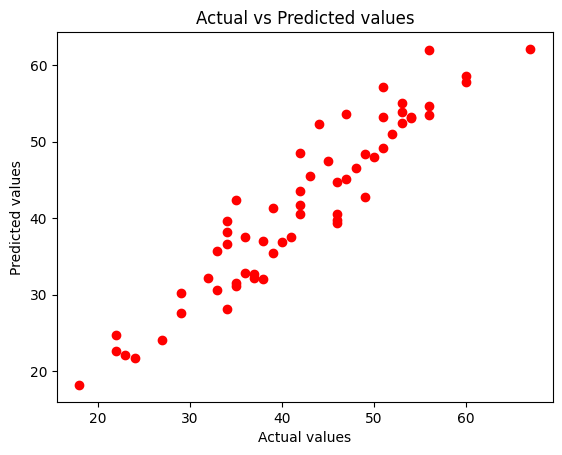
\includegraphics[keepaspectratio]{NBA_2023-24_files/figure-pdf/fig-predicted-output-1.png}}

}

\caption{\label{fig-predicted}Actual vs Predicted}

\end{figure}%

\textsubscript{Source:
\href{https://sigmadream.github.io/practice-quarto/NBA_2023-24.ipynb.html}{Article
Notebook}}

\phantomsection\label{refs}
\begin{CSLReferences}{1}{0}
\bibitem[\citeproctext]{ref-knuth84}
Knuth, Donald E. 1984. {``Literate Programming.''} \emph{Comput. J.} 27
(2): 97--111. \url{https://doi.org/10.1093/comjnl/27.2.97}.

\end{CSLReferences}




\end{document}
